\documentclass{article}
\usepackage{amsmath}
\usepackage{tikz}
\usetikzlibrary{matrix}

\begin{document}

\[
\mathcal{Z}(\mathbf{q}) =
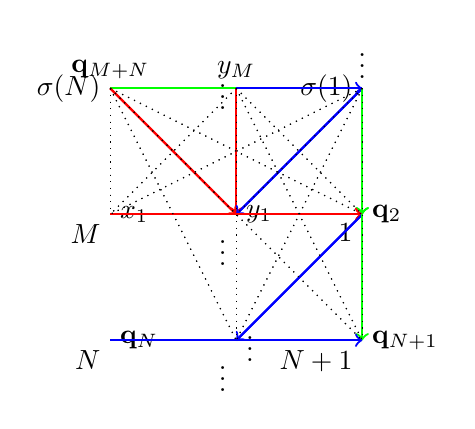
\begin{tikzpicture}[scale=0.8]
    % Define coordinates for the vertices
    \coordinate (A) at (-2,0);
    \coordinate (B) at (0,0);
    \coordinate (C) at (2,0);
    \coordinate (D) at (-2,-2);
    \coordinate (E) at (0,-2);
    \coordinate (F) at (2,-2);
    \coordinate (G) at (-2,-4);
    \coordinate (H) at (0,-4);
    \coordinate (I) at (2,-4);
    
    % Draw the horizontal lines
    \draw[thick, green] (A) -- (C);
    \draw[thick, blue] (B) -- (C);
    \draw[thick, red] (A) -- (E);
    \draw[thick, red] (B) -- (E);
    \draw[thick, blue] (C) -- (E);
    \draw[thick, green] (C) -- (F);
    \draw[thick, red] (D) -- (F);
    \draw[thick, red] (E) -- (F);
    \draw[thick, blue] (F) -- (H);
    \draw[thick, green] (F) -- (I);
    \draw[thick, blue] (G) -- (I);
    
    % Draw the vertical lines
    \draw[dotted] (A) -- (D);
    \draw[dotted] (B) -- (D);
    \draw[dotted] (C) -- (D);
    \draw[dotted] (A) -- (E);
    \draw[dotted] (B) -- (E);
    \draw[dotted] (C) -- (E);
    \draw[dotted] (A) -- (F);
    \draw[dotted] (B) -- (F);
    \draw[dotted] (C) -- (F);
    \draw[dotted] (A) -- (H);
    \draw[dotted] (B) -- (H);
    \draw[dotted] (C) -- (H);
    \draw[dotted] (A) -- (I);
    \draw[dotted] (B) -- (I);
    \draw[dotted] (C) -- (I);
    
    % Label the vertices
    \node at (A) [left] {$\sigma(N)$};
    \node at (B) [left] {$\vdots$};
    \node at (C) [left] {$\sigma(1)$};
    \node at (D) [below left] {$M$};
    \node at (E) [below left] {$\vdots$};
    \node at (F) [below left] {$1$};
    \node at (G) [below left] {$N$};
    \node at (H) [below left] {$\vdots$};
    \node at (I) [below left] {$N+1$};
    
    % Label the edges
    \node at (A) [above] {$\mathbf{q}_{M+N}$};
    \node at (B) [above] {$y_M$};
    \node at (C) [above] {$\vdots$};
    \node at (D) [right] {$x_1$};
    \node at (E) [right] {$y_1$};
    \node at (F) [right] {$\mathbf{q}_2$};
    \node at (G) [right] {$\mathbf{q}_N$};
    \node at (H) [right] {$\vdots$};
    \node at (I) [right] {$\mathbf{q}_{N+1}$};
    
    % Draw the arrows
    \draw[->, thick, green] (C) -- (F);
    \draw[->, thick, blue] (B) -- (C);
    \draw[->, thick, red] (A) -- (E);
    \draw[->, thick, red] (B) -- (E);
    \draw[->, thick, blue] (C) -- (E);
    \draw[->, thick, green] (C) -- (F);
    \draw[->, thick, red] (D) -- (F);
    \draw[->, thick, red] (E) -- (F);
    \draw[->, thick, blue] (F) -- (H);
    \draw[->, thick, green] (F) -- (I);
    \draw[->, thick, blue] (G) -- (I);
    
    % Draw the dotted lines
    \draw[dotted] (A) -- (D);
    \draw[dotted] (B) -- (D);
    \draw[dotted] (C) -- (D);
    \draw[dotted] (A) -- (E);
    \draw[dotted] (B) -- (E);
    \draw[dotted] (C) -- (E);
    \draw[dotted] (A) -- (F);
    \draw[dotted] (B) -- (F);
    \draw[dotted] (C) -- (F);
    \draw[dotted] (A) -- (H);
    \draw[dotted] (B) -- (H);
    \draw[dotted] (C) -- (H);
    \draw[dotted] (A) -- (I);
    \draw[dotted] (B) -- (I);
    \draw[dotted] (C) -- (I);
\end{tikzpicture}
\]

\end{document}